\chapter*{Example mapping}

\ifcontent
    Collaboration is at the heart of \emph{Deliberate Discovery}. One of the best techniques available is \emph{Example Mapping}, which is described in full at https://cucumber.io/blog/2015/12/08/example-mapping-introduction
    
    Let's consider this simple feature from a lending library:
    
    \begin{framed}
        At the library, it's free to take out books that are on the shelves, but there is a charge if you want to reserve an item that's currently on loan.
    
        The charges are:
    
        \begin{itemize}
            \item Adult membership - \$1.00 per item
            \item Child membership
                \begin{itemize}
                    \item Free for up to 6 children's books
                    \item 50c per item for all others
                \end{itemize}
        \end{itemize}
    \end{framed}
    
    The business have already prioritized this feature and have gathered the requirements. The picture below shows an incomplete Example Map, as it might look at the start of a collaboration session - the feature is written on a yellow card and the business rules are written on blue cards:
    
    \begin{center}
        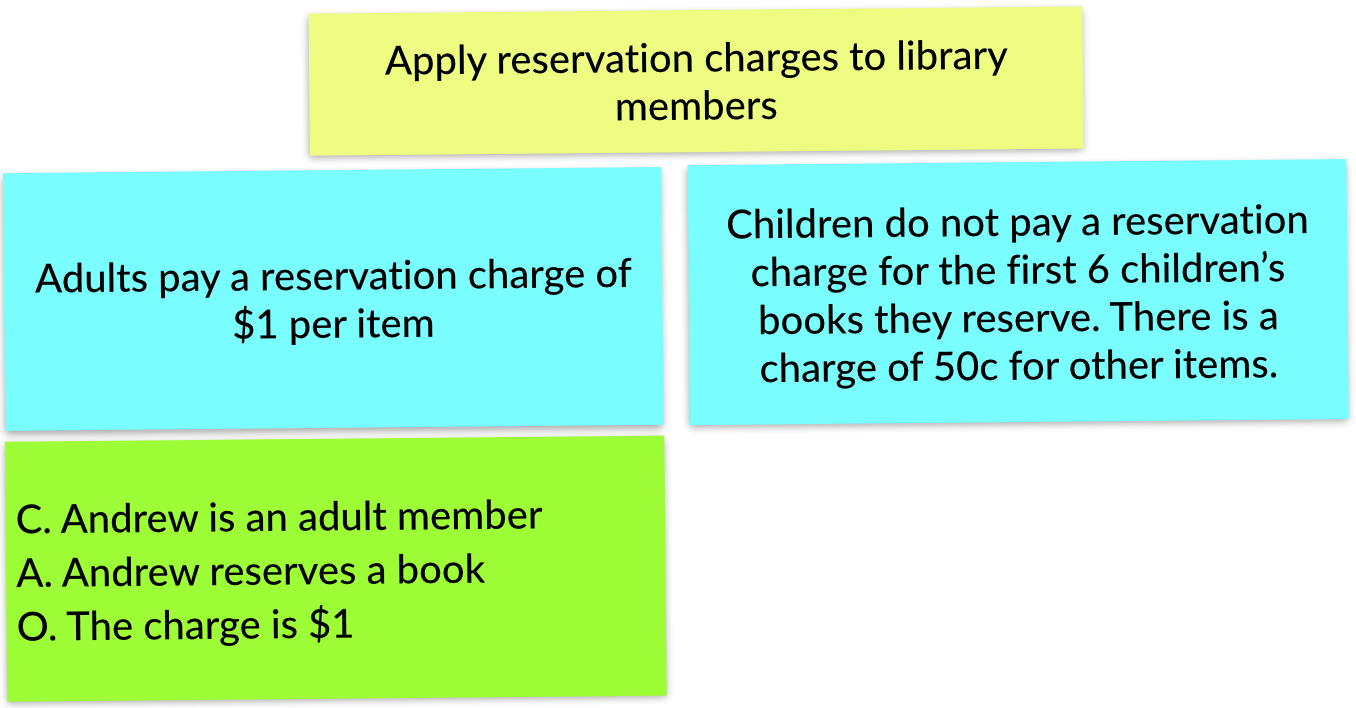
\includegraphics[width=0.55\textwidth, keepaspectratio]{images/library-example-map}
    \end{center}
    
    For each blue card in the map, we will create several \emph{concrete examples} of how the rule might work. One example might be: when an adult member reserves one book, then they should be charged \$1.
    
    We'll write each example on a green card and place it below the rule that it illustrates. 
    
    When you find yourselves asking a question that you don't have an answer to, we'll write this on a pink card.
    
    \QandAbox{What did we discover about the library requirements during the exercise?}{2}
\fi 
